%
% 02_konstruktion.tex -- Schrittweise Konstruktion des Beweises
%
% (c) 2026 Dominik Castelberg, Ostschweizer Fachhochschule
%
% !TEX root = ../../buch.tex
% !TEX encoding = UTF-8
%
\section{Konstruktion des Beweises
\label{jordan:section:konstruktion}}
\kopfrechts{Naive Ansätze für den Beweis}

\subsection{Der naive Ansatz Form-spezifischer Beweise}

Wie bereits erwähnt, ist der Satz von Jordan für spezielle Kurvenformen wie Kreise oder Ellipsen trivial zu beweisen.
So wäre der Beweis für eine Kreisform $\gamma(t) = (r \cos(2\pi t), r \sin(2\pi t))$ mit $t \in [0,1]$ und $r > 0$ einfach zu führen, da die Kurve die Ebene in ein inneres Gebiet (den Kreis) und ein äusseres Gebiet (die unendliche Fläche ausserhalb des Kreises) teilt.

\begin{proof}[Beweis des Jordan'schen Satzes für Kreise]
    Sei $\gamma(t) = (r \cos(2\pi t), r \sin(2\pi t))$ eine einfache geschlossene Kurve in der Ebene $\mathbb{R}^2$. 
    Das innere Gebiet $I$ ist definiert als die Menge aller Punkte $(x,y)$, die die Ungleichung $x^2 + y^2 < r^2$ erfüllen. 
    Das äussere Gebiet $A$ ist definiert als die Menge aller Punkte $(x,y)$, die die Ungleichung $x^2 + y^2 > r^2$ erfüllen. 
    Die Kurve $\gamma$ selbst bildet den gemeinsamen Rand dieser beiden Gebiete, da sie die Gleichung $x^2 + y^2 = r^2$ erfüllt.    
    Daher hält der Satz von Jordan für Kreise.
\end{proof}

\begin{figure}
    \centering
    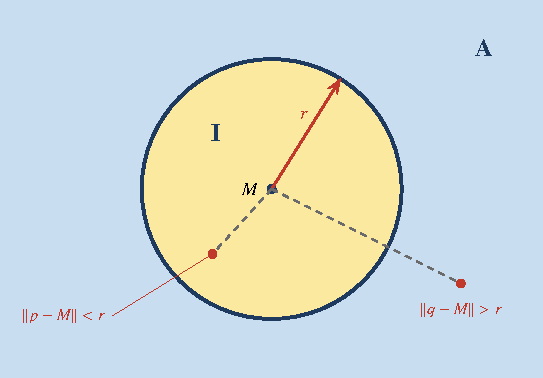
\includegraphics{papers/jordan/images/beweis_kreis.pdf}
    \caption{Aufteilung der Ebene $E$ durch eine Kreisform in ein inneres Gebiet $I$ und ein äusseres Gebiet $A$.}
\end{figure}

Doch dieser Beweis ist stark auf die spezielle Form der Kurve angewiesen und lässt sich nicht auf beliebige einfache geschlossene Kurven verallgemeinern. 
Da es potentiell unendlich viele verschiedene Formen von einfachen geschlossenen  Kurven gibt, ist es unmöglich, für jede Form einen eigenen Beweis zu führen. 
Dies macht den Ansatz form-spezifischer Beweise unpraktikabel und ineffizient.

\subsection{Beweis für konvexe Polygone\label{jordan:section:konvexe_polygone}}

Konvexe Polygone sind eine weniger restriktive Form von einfachen geschlossenen  Kurven. 
Der Beweis des Jordan'schen Satzes für konvexe Polygone kann aus der Definition der konvexen Hülle als Schnittmenge aller Halbebenen, die alle Eckpunkte des Polygons enthalten, abgeleitet werden.

\begin{definition}[Halbebene]
    Eine Halbebene in der Ebene $\mathbb{R}^2$ ist die Menge aller Punkte, die auf einer Seite einer Geraden liegen.
\end{definition}

\begin{definition}[Konvexe Hülle]
    Die konvexe Hülle einer Menge von Punkten $S$ in der Ebene $\mathbb{R}^2$ ist die kleinste konvexe Menge, die alle Punkte in $S$ enthält.
    Die Schnittmenge aller Halbebenen, die alle Punkte in $S$ enthalten, bildet die konvexe Hülle von $S$.
\end{definition}

\begin{figure}
    \centering
    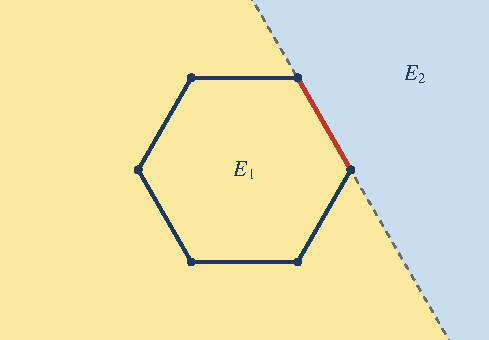
\includegraphics{papers/jordan/images/polygon_halbebene.pdf}
    \caption{Aufteilung der Ebene $E$ durch eine erweiterte Hexagonseite $g$ in zwei Halbebenen $E_1$ und $E_2$.}
\end{figure}


\begin{proof}[Beweis des Jordan'schen Satzes für konvexe Polygone]
    Sei $\gamma$ ein konvexes Polygon in der Ebene $\mathbb{R}^2$. 
    Das innere Gebiet $I$ ist die konvexe Hülle der Eckpunkte des Polygons, während das äussere Gebiet $A$ die Menge aller Punkte ausserhalb dieser Hülle ist. 
    Die Kurve $\gamma$ selbst bildet den gemeinsamen Rand dieser beiden Gebiete, da sie die Eckpunkte des Polygons verbindet. 
    Daher hält der Satz von Jordan für konvexe Polygone.
\end{proof}

Einfache geschlossene Kurven können jedoch auch nicht-konvexe Formen annehmen, was den Beweis für konvexe Polygone erneut unzureichend macht, um den Satz von Jordan im Allgemeinen zu beweisen.

\subsection{Beweis für einfache Polygone\label{jordan:section:einfache_polygone}}

Einfache Polygone verwerfen die Einschränkng der Konvexität und erlauben es, dass die Kurve in sich selbst zurückkehrt, solange sie sich nicht schneidet. 
Die Eigenschaft der Konvexität war jedoch in der vorherigen Beweisführung entscheidend, da sie die Definition der konvexen Hülle und die Trennung der Ebene in zwei Gebiete erleichtert hat. 

Wir benötigen daher einen neuen Ansatz, um die bisherigen, durch die Eigenschaften der Konstruktion der behandelten Körper gegebenen, Definitionen für ``Innen'' und ``Aussen'' neu zu formulieren. Ein wertvolles Werkzeug ist hierbei die Strahlenparität.

\begin{definition}[Strahlenparität]
    Sei $P$ ein einfaches Polygon und $p \in \mathbb{R}^2 \setminus \partial P$.
    Für jeden strahl $L$ mit Anfangspunkt $p$, der keine Ecke von $P$ trifft und nicht entlang einer Kante von $P$ verläuft, sei $N(p,L)$ die Anzahl Schnittpunkte von $L$ mit $\partial P$. 
    Dann gilt:
    \begin{itemize}
        \item $N(p,L)$ ist endlich.
        \item Die Parität von $N(p,L)$ hängt nicht von $L$ ab, sondern nur von $p$.
    \end{itemize}
\end{definition}

\begin{figure}
    \centering
    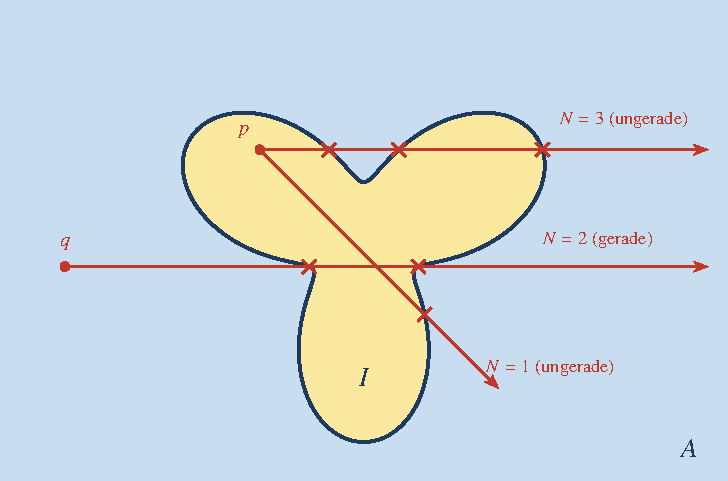
\includegraphics{papers/jordan/images/strahlenparitaet.pdf}
    \caption{Strahlenparität am Beispiel einer Jordan-Kurve.}
\end{figure}


Diese Definition erlaubt es, die Punkte in der Ebene in zwei Mengen zu unterteilen: diejenigen, die eine gerade Anzahl von Schnittpunkten mit dem Polygon haben (die äussere Menge), und diejenigen, die eine ungerade Anzahl von Schnittpunkten haben (die innere Menge).

\begin{definition}[Innen- und Aussengebiet]
    Sei $P$ ein einfaches Polygon und $p \in \mathbb{R}^2 \setminus \partial P$. 
    Dann gilt:
    \begin{itemize}
        \item $p$ liegt im inneren Gebiet $I$ von $P$, wenn $N(p,L)$ ungerade ist.
        \item $p$ liegt im äusseren Gebiet $A$ von $P$, wenn $N(p,L)$ gerade ist.
    \end{itemize}
\end{definition}

Um den Satz von Jordan rigoros zu beweisen, müssen wir jedoch noch folgende Punkte zeigen:

\begin{itemize}
    \item $I$ und $A$ sind beide offen und nicht leer.
    \item $I$ und $A$ sind wegzusammenhängend.
    \item $I$ ist beschränkt, während $A$ unbeschränkt ist.
    \item $\partial P$ ist der gemeinsame Rand von $I$ und $A$.
\end{itemize}

\begin{lemma}[Offenheit von $I$ und $A$]
    Die Parität $N(p,L)$ ändert sich nicht, wenn $p$ innerhalb einer kleinen Umgebung verschoben wird, solange $p$ nicht auf $\partial P$ liegt. 
    Daher sind $I$ und $A$ offen.
\end{lemma}

\begin{lemma}[Nicht-Leerheit von $I$]
    Per Definition kann $I$ nicht leer sein, da Polygone mindestens drei Eckpunkte besitzen müssen, die ein inneres Gebiet definieren. 
    Daher ist $I$ nicht leer.
\end{lemma}

\begin{lemma}[Nicht-Leerheit von $A$]
    Die Absenz von $A$ ist unmöglich, da die Ebene $\mathbb{R}^2$ unbeschränkt ist und es daher immer Punkte gibt, die ausserhalb des Polygons liegen.
    Daher ist $A$ nicht leer.
\end{lemma}

Die Etablierung des Wegzusammenhangs von $I$ und $A$ verlangt ein topologisch substantielleres Argument: Die Wegzusammenhangseigenschaften von triangulierten Polygonen. 

\begin{definition}[Triangulierung eines einfachen Polygons]
    Eine Triangulierung eines einfachen Polygons $P$ ist eine Zerlegung von $P$ in nicht überlappende Dreiecke, deren Ecken jeweils Ecken von $P$ sind und die sich paarweise nur in Kanten oder Ecken schneiden.
\end{definition}

\begin{lemma}[Triangulierungssatz für einfache Polygone]
    Jedes einfache Polygon $P$ mit $n \geq 3$ Ecken besitzt eine Triangulierung.
\end{lemma}

%TODO Citation
Dieser Triangulierungssatz wurde 1975 von G. H. Meister präzise bewiesen. Der Beweis basiert auf folgendem Lemma:

\begin{lemma}[Existenz einer Diagonale]
    Jedes einfache Polygon $P$ mit $n \geq 4$ Ecken besitzt eine Diagonale, d.h. eine Linie, die zwei nicht benachbarte Ecken von $P$ verbindet und vollständig innerhalb von $P$ liegt.
\end{lemma}

Die Existenz einer in einem Polygon mit mehr als drei Ecken liegenden Diagonale impliziert, dass das Polygon in zwei kleinere Polygone zerlegt werden kann.

\begin{figure}
    \centering
    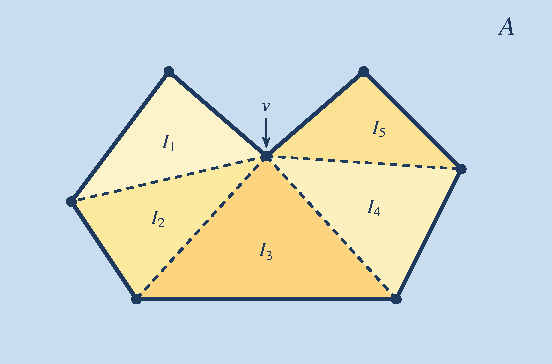
\includegraphics{papers/jordan/images/triangulierung.pdf}
    \caption{Triangulierung eines einfachen Polygons in nicht überlappende Dreiecke an Reflexpunkt $v$.}
\end{figure}

\begin{lemma}[Wegzusammenhang von $I$]
    Sei $P$ ein einfaches Polygon und $I$ das innere Gebiet von $P$. 
    Der Triangulierungssatz für einfache Polygone garantiert, dass jedes $P$ mit $n \geq 3$ Ecken in nicht überlappende Dreiecke zerlegt werden kann.
    Da Dreiecke als konvexe Polygone wegzusammenhängend sind, können wir einen Weg zwischen zwei Punkten in $I$ konstruieren, indem wir die Dreiecke durchqueren, die das Polygon bilden.
    Daher ist $I$ wegzusammenhängend.
\end{lemma}

\begin{lemma}[Wegzusammenhang von $A$]
    Sei $P$ ein einfaches Polygon, $I$ das innere Gebiet von $P$, $A$ das äussere Gebiet von $P$, und $K$ das innere Gebiet eines Kreises, welche $P$ umschliesst, ohne es zu berühren, und $A$ das äussere Gebiet von $P$. 
    Da $A$ unbeschränkt ist, können wir einen Weg von einem Punkt $k \in K \setminus P \cup I$ zu einem Punkt $a \in A$ konstruieren, der keine Punkte von $P$ enthält. 
    Daher ist $A$ wegzusammenhängend.
\end{lemma}

\begin{lemma}[Beschränktheit von $I$]
    Sei $P$ ein einfaches Polygon und $I$ das innere Gebiet von $P$. 
    Da $P$ eine endliche Anzahl von Ecken hat, ist die konvexe Hülle von $P$ beschränkt. 
    Daher ist auch $I$ beschränkt.
\end{lemma}

\begin{lemma}[Unbeschränktheit von $A$]
    Sei $P$ ein einfaches Polygon und $A$ das äussere Gebiet von $P$. 
    Da die Ebene $\mathbb{R}^2$ unbeschränkt ist, gibt es immer Punkte, die ausserhalb der konvexen Hülle von $P$ liegen. 
    Daher ist $A$ unbeschränkt.
\end{lemma}



\begin{proof}[Gemeinsamer Rand von $I$ und $A$]
    Sei $P$ ein einfaches Polygon, $I$ das innere Gebiet von $P$, und $A$ das äussere Gebiet von $P$.
    Die Kurve $\partial P$ bildet einen gemeinsamen Rand von $I$ und $A$, da jeder Punkt auf $\partial P$ sowohl adjazent zu Punkten in $I$ als auch adjazent zu Punkten in $A$ liegt.
    Sie ist die einzige gemeinsame Rand, da $I$ per Definition durch $P$ begrenzt ist.
\end{proof}

In Kombination führen diese Lemmas und Definitionen zu einem vollständigen Beweis des Jordan'schen Satzes für einfache Polygone.

%TODO: Ausformulierung Beweis

\subsection{Beweis für Reell-analytische Kurven}

Mit dem Schritt von einfachen Polygonen zu reell-analytischen Kurven (im Folgenden als $\gamma$ bezeichnet) verlieren wir mehrere Eigenschaften und Werkzeuge, welche wir bisher für die Beweisführung verwendet haben. 

Spezifisch verlieren wir:

\begin{itemize}
    \item \textbf{Strahlenparität:} Die Zahl der Schnittpunkte eines Strahls mit $\gamma$ ist nicht mehr offensichtlich endlich, da $\gamma$ keine Kanten mehr hat. 
    \item \textbf{Triangulierung:} Es gibt keine kanonische Triangulierung von $I$ mit Ecken auf $\gamma$, weil $\gamma$ keine Ecken hat. 
    \item \textbf{Diagonal-Lemma:} Aus dem gleichen Grund ist das Konzept einer Diagonale nicht mehr anwendbar, da $\gamma$ keine Ecken hat.
\end{itemize}

Entsprechend stehen wir vor einer Wegzweigung: Entweder wir erweitern das Werkzeug der Strahlenparität, sodass es auf reell-analytische Kurven anwendbar ist, oder wir finden ein neues Werkzeug, das die Strahlenparität ersetzt. 
Wir werden in diesem Abschnitt beide Ansätze diskutieren dabei herausfinden, dass einer der Ansätze dabei deutlich eleganter ist. 

Zusätzlich erhalten wir dank der Reell-Analytizität von $\gamma$ eine neue Kiste von analytischen Werkzeugen, die wir für unsere Beweisführung verwenden können:

\subsubsection{Fortführung des Strahlenparität-Arguments}

Um die Strahlenparität weiter zu entwickeln, betrachten wir die Wirkung von Deformationen auf die Anzahl der Schnittpunkte zwischen einer Kurve und einem Strahl. 
Hierfür verwenden wir zwei neue, analytische Werkzeuge: Die endliche Schnittstruktur und die Tubulare Umgebung. 

\begin{satz}[Endliche Schnittstruktur]
    Sei $\gamma$ eine reell-analytische Kurve in der Ebene $\mathbb{R}^2$ und $L$ ein Strahl mit Anfangspunkt $p \in \mathbb{R}^2$.
    Dann ist $\gamma \cap L$ endlich. Ausnahmefall ist $\gamma \cap L = \emptyset$.
\end{satz}

\begin{satz}[Identitätssatz für reell-analytische Funktionen]
    Sei $f: U \subset \mathbb{R} \to \mathbb{R}$ eine nicht verschwindende reell-analytische Funktion auf einer zusammenhängenden Menge $U$.
    Die Nullstellen von $f$ auf $U$ sind diskret und auf einer kompakten Teilmenge von $U$ somit endlich.
\end{satz}

Da $\gamma \cap L = \emptyset$ bei geschlossenen Kurven nicht auftreten kann, und der Satz von Jordan eine geschlossene Kurve $\gamma$ voraussetzt, gilt der Satz der endlichen Schnittstruktur für sämtliche für uns relevanten Kurven. 

\begin{proof}[Beweis der endlichen Schnittstruktur]

    Gegeben sei eine reell-analytische Kurve $\gamma$ in der Ebene $\mathbb{R}^2$ und ein Strahl $L$ mit Anfangspunkt $p \in \mathbb{R}^2$. 
    Da $\gamma$ reell-analytisch ist, existiert eine reell-analytische Funktion $f: U \subset \mathbb{R}^2 \to \mathbb{R}$, die $\gamma$ lokal beschreibt. 
    Die Schnittpunkte von $\gamma$ und $L$ entsprechen den Nullstellen von $f$ auf $L$. 
    Da $f$ nicht verschwindend ist und $L$ eine zusammenhängende Menge ist, folgt aus dem Identitätssatz für reell-analytische Funktionen, dass die Nullstellen von $f$ auf $L$ diskret sind. 

    Entsprechend ist die Menge der Schnittpunkte $\gamma \cap L$ endlich, da eine diskrete Menge auf einer kompakten Teilmenge von $L$ nur endlich viele Punkte enthalten kann.
\end{proof}

\begin{proof}[Beweis des Identitätssatzes für reell-analytische Funktionen]

\end{proof}

Mit der endlichen Schnittstruktur können wir garantieren, dass die Anzahl der Schnittpunkte zwischen einem Strahl und einer reell-analytischen Kurve endlich ist. 
Dies ist ein wichtiger Schritt in der Fortführung des Strahlenparitäts-Arguments, da mit der Modulo-Rechnung unser Mittel, die Parität der Schnittpunkte zu analysieren, nur auf endliche Mengen anwendbar ist. 

Mit dem Beweis der endlichen Schnittstruktur abgeschlossen, können wir nun die Tubulare Umgebung einführen, die es uns erlaubt, die Strahlenparität auf reell-analytische Kurven zu erweitern.

\begin{lemma}[Tubulare Umgebung]
    Sei $\gamma$ eine reell-analytische Kurve in der Ebene $\mathbb{R}^2$. Dann existiert $\varepsilon > 0$, so dass die Abbildung $\varphi: S\textsuperscript{1} \times (-\varepsilon, \varepsilon) \to \mathbb{R}^2$, $\varphi(t,s) = \gamma(t) + s \cdot n(t)$, ein reell-analytischer Diffeomorphismus auf eine offene Umgebung $T$ von $\gamma$ ist, wobei $n(t)$ der nach aussen gerichtete Einheitsnormalenvektor ist. 
    Das Komplement $T \setminus \gamma$ zerfällt in zwei zusammenhängende Komponenten entsprechend $s > 0$ und $s < 0$, die als innere und äussere tubulare Umgebung bezeichnet werden.    
\end{lemma}

\begin{figure}
    \centering
    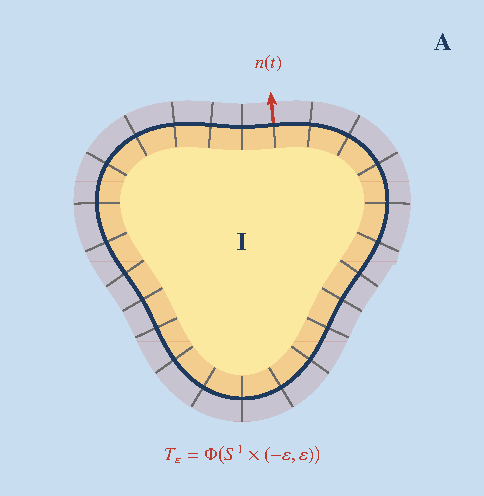
\includegraphics{papers/jordan/images/tubulare_umgebung.pdf}
    \caption{Die tubulare Umgebung einer reell-analytischen Kurve.}
\end{figure}

Das Lemma der tubularen Umgebung kann mithilfe der Determinanten der im Abschnitt \ref{buch:holomoprh:holomorph:subsection:komplexedifferenzierbarkeit} eingeführten Jacobi-Matrix bewiesen werden.  

\begin{proof}[Beweis des Lemmas der tubulären Umgebung]
    Sei $\gamma$ eine reell-analytische Kurve in der Ebene $\mathbb{R}^2$ und $\varphi$ die durch $\varphi(t,s) = \gamma(t) + s \cdot n(t)$ definierte Abbildung. 
    Die Jacobi-Determinante von $\varphi$ in $(t,0)$ ist $||\gamma'(t)|| \neq 0$. 
    Nach dem Satz über die Umkehrfunktion ist $\varphi$ lokal ein Diffeomorphismus um jeden Punkt $(t,0)$. 
    Globale Injektivität auf einem Streifen $S\textsuperscript{1} \times (-\epsilon, \epsilon)$ folgt aus der Kompaktheit und der Einfachheit von $\gamma$: 
    Wäre $\varphi(t_1,s_1) = \varphi(t_2,s_2)$ für $(t_1,s_1) \neq (t_2,s_2)$, so würde dies bedeuten, dass $\gamma(t_1) + s_1 n(t_1) = \gamma(t_2) + s_2 n(t_2)$, was im Widerspruch zur Injektivität von $\gamma$ steht.
\end{proof}

Mit diesen beiden Werkzeugen können wir die Strahlenparität auf reell-analytische Kurven erweitern und somit den Beweis des Satzes von Jordan für diese Kurven fortsetzen. 

\begin{lemma}[Satz von Jordan für reell-analytische Kurven]
    Der Satz von Jordan gilt auch für reell-analytische, einfache geschlossene Kurven in der Ebene $\mathbb{R}^2$.
\end{lemma}

Wir können nun den polygonalen Beweis als Grundlage verwenden und die Strahlenparität mit den zuvor bewiesenen Lemmas erweitern.

\begin{proof}[Beweis des Satzes von Jordan für reell-analytische Kurven]
    Für $p \in \mathbb{R}^2 \setminus \gamma$ wählen wir einen Strahl $L$ mit Anfangspunkt $p$, der nicht tangential an $\gamma$ verläuft und durch keinen degenerierten Punkt von $\gamma$ geht.
    Nach dem Lemma der endlichen Schnittstruktur ist die Anzahl der Schnittpunkte $N(p,L)$ diskret, also ist jede Richtung zulässig. 
    Sei N(p,L) die Anzahl der Schnittpunkte von $L \cap \gamma$. Nach dem Satz der endlichen Schnittstruktur ist ist diese Zahl endlich. 
    Die Parität $N(p,L) \mod 2$ ist wohldefiniert und hängt nicht von der Wahl des Strahls ab. 
    Der Wegzusammenhang von $I$ und $A$ und die Beschränktheit von $I$ ergeben sich aus der Konstruktion der tubulären Umgebung. 
    Die Beweise der Offenheit von $I$ und $A$, genauso wie die Unbeschränktheit von $A$, haben sich nicht verändert.
    Daher gilt der Satz von Jordan auch für reell-analytische, einfache geschlossene Kurven in der Ebene $\mathbb{R}^2$.
\end{proof}

Dieser Beweis funktioniert, aber leider ist er auch analytisch aufwendig:

\begin{itemize}
    \item Fallunterscheidung zu Tangentenschnitten
    \item Kontrolle der Paritätsinvarianz unter Strahlendeformationen
    \item Genaue Analyse entarteter Strahlrichtungen
\end{itemize}

All diese Punkte verlangen sorgfältige analytische Arbeit, welche im polygonalen Fall durch die kombinatorische Endlichkeit ersetzt war. 
Entsprechend werden wir uns nun einem alternativen Ansatz, der uns mit seiner Eleganz viel Arbeit erspart, zuwenden. 

\subsubsection{Nutzung der Umlaufzahl statt der Strahlenparität}

Im Abschnitt \ref{buch:integration:cauchy:subsetion:umlaufzahl} wurde die Umlaufzahl eines Weges um einen Punkt eingeführt. 
Diese Umlaufzahl besitzt Eigenschaften, die es uns erlauben, die Strahlenparität als Argument komplett zu verwerfen. 

\begin{lemma}[Grundlegende Eigenschaften der Umlaufzahl]
    Für jede geschlossene, stückweise C\textsuperscript{1}-Kurve $\gamma$ mit Umlaufzahl $n(\gamma, z)$ und $z \notin \gamma$ gilt:
    \begin{enumerate}
        \item $n(\gamma, z) \in \mathbb{Z}$
        \item Die Abbildung $z \mapsto n(\gamma, z)$ ist lokal konstant auf $\mathbb{C} \setminus \gamma$.
        \item Für $|z|$ hinreichend gross gilt $n(\gamma, z) = 0$.
    \end{enumerate}

\end{lemma}

\begin{proof}[Beweis der grundlegenden Eigenschaften der Umlaufzahl]
    \begin{enumerate}
        \item Man betrachte die Funktion $F(s) = exp(\int_0^s \frac{\gamma'(t)}{\gamma(t) - z} dt)$. 
            Differenzieren zeigt $\frac{F'(s)}{F(s)} = \frac{\gamma'(s)}{\gamma(s) - z}$. 
            Zugleich ist $\frac{d}{ds} \frac{[\gamma(s) -z]}{[\gamma(0) -z]} = \frac{\gamma'(s)}{\gamma(0) - z}$ und ein Vergleich zeigt, dass $F(s) \cdot [\gamma(0) - z] = \gamma(s) -z$. 
            Im Falle von $s = 1$ erhalten wir $F(1) \cdot [\gamma(0) - z] = \gamma(1) -z = \gamma(0) - z$, also $F(1) = 1$.
            Daher gilt $\int_0^1 \frac{\gamma'(t)}{\gamma(t) - z} dt = 2 \pi i n$ für ein $n \in \mathbb{Z}$.
        \item Der Integrand $z \mapsto \frac{1}{\zeta - z}$ ist stetig in $z$ und gleichmässig auf $\gamma$, da $\gamma$ kompakt ist und $|\zeta - z|$ von unten beschränkt bleibt für $z$ in Kompakta von $\mathbb{C} \setminus \gamma$. 
            Daher ist $n(\gamma, \cdot)$ stetig in $z$ und als stetige ganzzahlige Funktion lokal konstant.
        \item Für $|z| \gg sup |\gamma|$ kann man unter dem Integral abschätzen: 
            \[
                \left| \frac{\gamma'(t)}{\gamma(t) - z} \right| \leq \frac{|\gamma'(t)|}{|z| - |\gamma(t)|} \leq \frac{|\gamma'(t)|}{|z| - sup |\gamma|}.
            \]
            Da $|\gamma'(t)|$ integrierbar ist, folgt, dass das Integral gegen null geht, wenn $|z|$ gegen unendlich geht. 
            Daher gilt $n(\gamma, z) = 0$ für $|z|$ hinreichend gross.
    \end{enumerate}
\end{proof}

Aus diesen Eigenschaften folgt schon fast der Satz von Jordan im analytischen Fall: Die Funktion $z \mapsto n(\gamma, z)$ nimmt auf jeder zusammenhängenden Komponente von $\mathbb{C} \setminus \gamma$ einen konstanten ganzzahligen Wert an. 
Auf der unbeschränkten Komponente ist dieser Wert $0$. 

Für einen vollständigen Beweis müssen wir jedoch noch zeigen, dass es mindestens eine Komponente gibt, auf der $n(\gamma, z) \neq 0$ gilt und dass es auf jeder beschränkten Komponente den Wert $\pm 1$ gibt.

\begin{satz}[Hopfscher Umlaufsatz]
    Für jede einfach geschlossene reguläre C\textsuperscript{1}-Kurve $\gamma$ ist die Totaldrehung $\pm 1$. 
\end{satz}

%TODO Tangentenwindungszahl
\begin{figure}
    \centering
    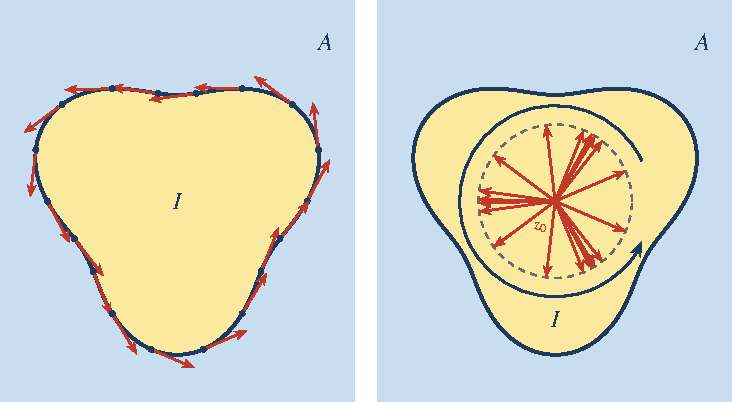
\includegraphics{papers/jordan/images/tangentenwindungszahl.pdf}
    \caption{Drehung der Tangenten beim Umlauf einer Kurve (links). Die Nettodrehung der Tangentenvektoren $\tau(t)$ entlang der Kurve $\gamma$ ist $2\pi$, was der Umlaufzahl $n(\gamma, z_0) = 1$ entspricht (rechts).}
\end{figure}

%TODO Hopfscher Umlaufsatz

\begin{figure}
    \centering
    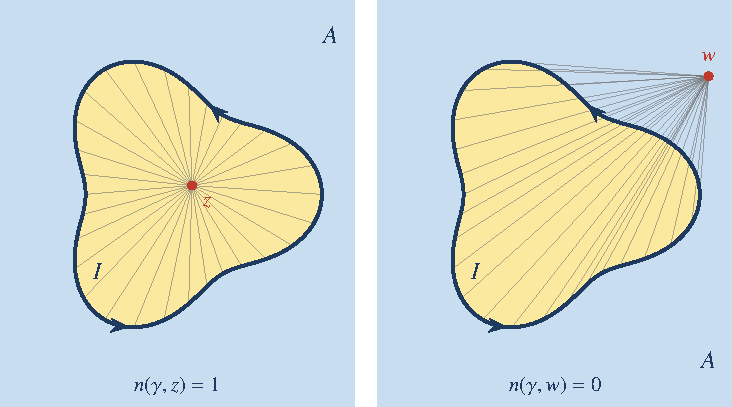
\includegraphics{papers/jordan/images/umlaufzahl.pdf}
    \caption{Konstruktion der Umlaufzahl am Beilspiel eines Punkts innerhalb (links) und ausserhalb (rechts) einer Jordan-Kurve.}
\end{figure}

\subsection{Beweis für Stückweise $C\textsuperscript{1}$-Kurven}

\begin{figure}
    \centering
    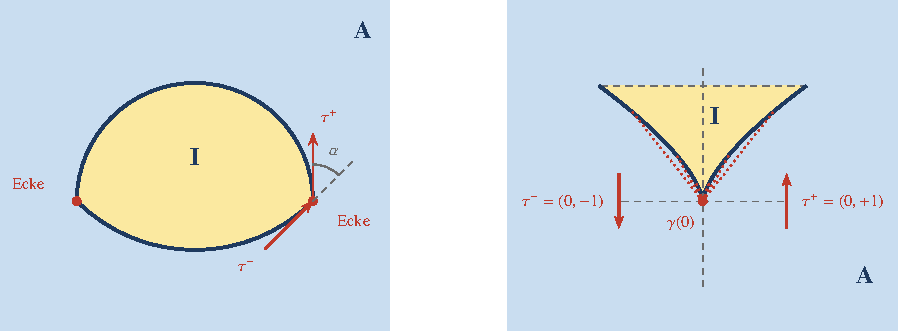
\includegraphics{papers/jordan/images/spitzen_ecken.pdf}
    \caption{Tangentenrichtung springt an Ecken (links) und kehrt an Spitzen (rechts).}
\end{figure}

%TODO Gauss-Bonnet Modifikation

\subsection{Beweis für Stetige Kurven}

\begin{figure}
    \centering
    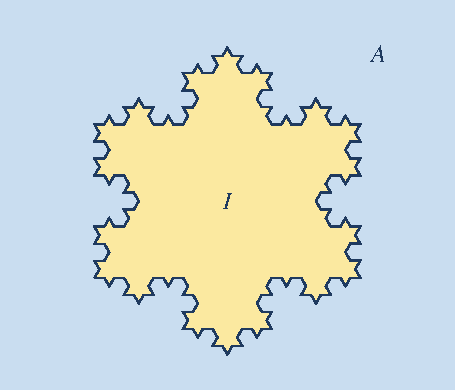
\includegraphics{papers/jordan/images/koch_schneeflocke.pdf}
    \caption{Koch-Schneeflocke als Beispiel für ein Fraktal, dargestellt mit Iterationstiefe 3.}
\end{figure}

%TODO Warum habe ich so viel Zeit damit verbracht, über Polygone zu reden? "Aufmerksame Leser fragen sich..."

\begin{figure}
    \centering
    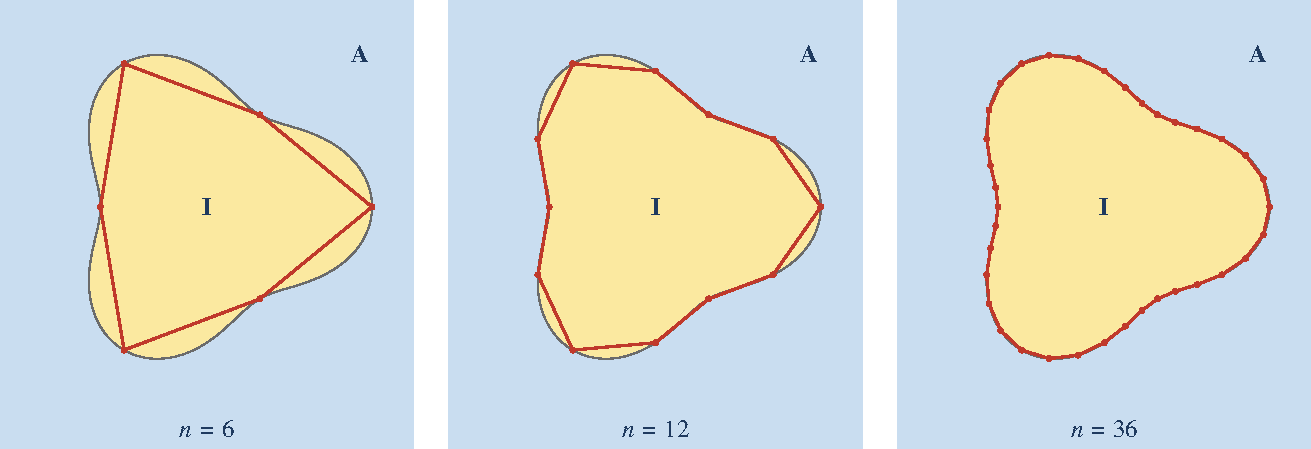
\includegraphics{papers/jordan/images/polygonale_approximation.pdf}
    \caption{Polygonale Approximation einer stetigen Kurve.}
\end{figure}

%TODO Approximierung durch einfache Polygone (lokale Approximation)

%TODO Überleitung zur Alexander-Dualität